\section{Experiments}

\subsection{Data}
We scan 267 AntAWS 3-hourly station files and retain stations with record length of at least 10 years, temperature completeness of at least 70\%, mean core-variable completeness of at least 50\%, and minimum core-variable completeness of at least 20\%. This yields 27 main stations and five held-out stations: Butcher Ridge, Mount Sidley, Nico, Sabrina, and Zhongshan. ERA5 point time series are aligned to the exact station timestamps and normalized with statistics fitted on main-station train windows.

\begin{figure}[t]
  \centering
  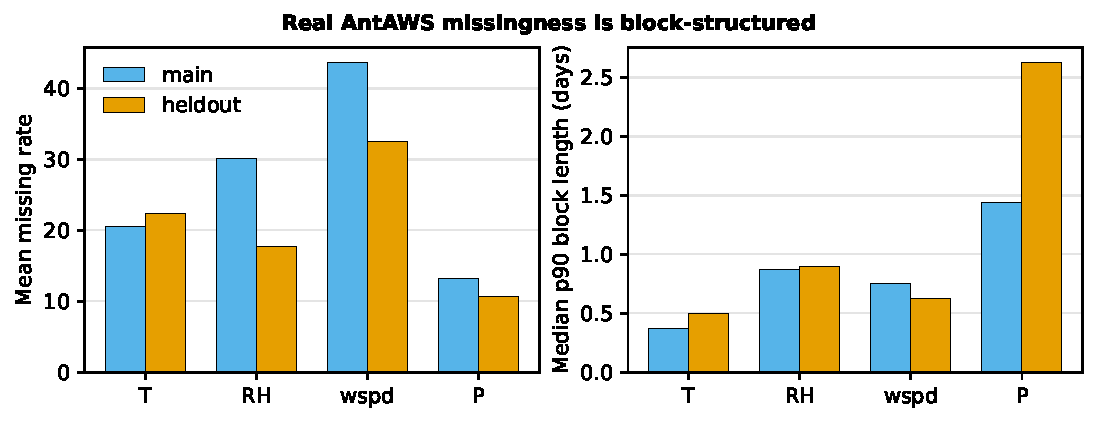
\includegraphics[width=\columnwidth]{figures/fig_missing_patterns.pdf}
  \caption{Observed missingness in selected AntAWS stations. Wind speed and relative humidity show the largest missing burden, and high-percentile gaps last multiple days, motivating block-wise rather than point-wise imputation.}
  \label{fig:missing-patterns}
\end{figure}

\subsection{Baselines and Ablations}
Round 1 compares six baselines: linear interpolation, last-observation-carried-forward, ERA5 direct substitution after train-set bias correction, BRITS, SAITS, and an iTransformer imputation baseline. Round 2 evaluates ECBIT variants: full conditional cross-attention, no cross-attention, no ERA5, and no block-mask training. Round 3 evaluates held-out station generalization for ECBIT full at a 40\% missing rate.

\subsection{Implementation Status}
The data pipeline, model implementations, training/evaluation entrypoints, and 315 YAML experiment configurations have been implemented. Remote GPU execution is pending SSH credential availability. Result tables and statistical comparisons will be added after the remote experiment batches complete.
